%% =============================================================================
%% SWR_v4_en.tex -- English version
%% Synthetic Worldview Reconstruction: A Method for LLM-Assisted
%% Group-Level Belief System Analysis
%% Autor: Lukas Geiger, Independent Researcher, Bernau
%% Paper B v4.0 -- Source-check maintenance version
%% Reference baseline: Paper A v8.0 live Zenodo version
%% =============================================================================
\documentclass[11pt,a4paper]{article}

%% --- Encoding and Language ---------------------------------------------------
\usepackage{cmap}
\usepackage[utf8]{inputenc}
\usepackage[T1]{fontenc}
\input{glyphtounicode}
\pdfgentounicode=1
\makeatletter
\@ifundefined{pdftracingfonts}{}{\pdftracingfonts=1}
\makeatother
\usepackage[english]{babel}
\usepackage{microtype}

%% --- Fonts: Latin Modern + Helvetica -----------------------------------------
\usepackage{lmodern}
\usepackage[scaled=0.92]{helvet}

%% --- Page Layout -------------------------------------------------------------
\usepackage[left=2.5cm, right=2.5cm, top=2.5cm, bottom=2.5cm]{geometry}

%% --- Line Spacing: 1.5 ------------------------------------------------------
\usepackage{setspace}
\onehalfspacing
\emergencystretch=3em
\sloppy
\clubpenalty=10000
\widowpenalty=10000
\displaywidowpenalty=10000
\renewcommand{\topfraction}{0.85}
\renewcommand{\bottomfraction}{0.85}
\renewcommand{\textfraction}{0.10}
\renewcommand{\floatpagefraction}{0.80}


%% --- Section Headings: sans-serif --------------------------------------------
\usepackage{titlesec}
\titleformat{\section}
  {\normalfont\Large\bfseries\sffamily}{\thesection.}{0.5em}{}
\titleformat{\subsection}
  {\normalfont\large\bfseries\sffamily}{\thesubsection}{0.5em}{}
\titleformat{\subsubsection}
  {\normalfont\normalsize\bfseries\sffamily}{\thesubsubsection}{0.5em}{}

%% --- Citations: natbib -------------------------------------------------------
\usepackage[round,authoryear,semicolon]{natbib}

%% --- Packages ----------------------------------------------------------------
\usepackage{graphicx}
\usepackage{booktabs}
\usepackage{array}
\usepackage{multirow}
\usepackage{tabularx}
\usepackage{longtable}
\usepackage{amsmath,amssymb}
\usepackage{enumitem}
\usepackage{xcolor}
\usepackage{tikz}
\usetikzlibrary{arrows.meta,positioning,shapes.geometric,fit,backgrounds,calc}
\usepackage{xurl}
\usepackage[unicode=true,breaklinks=true]{hyperref}
\makeatletter
\renewcommand*{\HyperDestNameFilter}[1]{swrb-en-#1}
\makeatother
\newcolumntype{Y}{>{\raggedright\arraybackslash}X}
\newcolumntype{L}[1]{>{\raggedright\arraybackslash}p{#1}}
\newenvironment{promptquote}{%
  \begin{quote}\footnotesize\ttfamily\raggedright\sloppy
}{%
  \end{quote}
}
\newcommand{\backmatterlabel}[1]{%
  \par\smallskip
  \noindent\textbf{#1}\enspace
}
\setlength{\emergencystretch}{1.5em}
\hypersetup{
  unicode             = true,
  pdfencoding         = auto,
  bookmarksnumbered   = true,
  bookmarksopen       = true,
  pdfpagemode         = UseOutlines,
  pdfstartview        = {FitH},
  plainpages          = false,
  pdflang             = {en-US},
  breaklinks          = true,
  colorlinks          = true,
  linkcolor           = black,
  citecolor           = blue!60!black,
  urlcolor            = blue!70!black,
  pdfauthor           = {Lukas Geiger},
  pdftitle            = {Synthetic Worldview Reconstruction: A Method for LLM-Assisted Group-Level Belief System Analysis},
  pdfsubject          = {Computational Social Science, Methodology},
  pdfkeywords         = {synthetic worldview reconstruction, LLM-assisted methodology, collective belief systems, ideal type, group-level analysis, computational social science, inter-instance reliability},
}

%% --- Title Block -------------------------------------------------------------
\title{%
  \sffamily\bfseries
  Synthetic Worldview Reconstruction:\\[0.3em]
  \large A Method for LLM-Assisted Group-Level\\
  Belief System Analysis%
}

\author{%
  Lukas Geiger\thanks{Corresponding author: Lukas Geiger, Bernau, Germany. ORCID: \url{https://orcid.org/0009-0005-7296-1534}}\\[0.3em]
  \small Independent Researcher, Bernau, Germany
}

\date{October 2026}

%% =============================================================================
\begin{document}

\hypersetup{pageanchor=false}
\maketitle
\thispagestyle{empty}

%% --- Abstract ----------------------------------------------------------------
\begin{abstract}
\noindent
This paper presents \emph{Synthetic Worldview Reconstruction} (SWR)---a method for reconstructing the collective belief systems of sociologically defined groups using large language models. SWR formulates worldview analysis as an inverse problem: given the aggregated public statements and documented actions of a group, it reconstructs the latent belief system that most coherently accounts for those outputs. The method constructs a \emph{fictive synthetic person}---a Weberian ideal type---whose worldview represents the group's collective beliefs in distilled form. This paper abstracts SWR from its original application (a study of 100 influential AI actors; Geiger, 2026) into a transferable methodological framework. We describe the five-step protocol, the dimensional rating procedure as one operationalization example, and the focus control infrastructure. The pilot records five group profiles with two repetitions each: the historical mean of one-way coefficients and a separate two-way absolute-agreement calculation both round to 0.902; the latter is a descriptive profile index without a bound population uncertainty model. A separate $N$\,=\,15 protocol reports ICC(3,1)\,=\,0.847 for single-measure consistency and ICC(2,k)\,=\,0.988 for agreement of its 15-run mean. Cross-modal prediction records 72\% confirmed and 0\% contradicted in that pilot; the tabulated placeholder-versus-fictional-name profiles yield Pearson $r$\,=\,0.9585 and MAE\,=\,0.33. These local observations do not establish external construct validity or general equivalence of blinding strategies. Tiered acceptance criteria distinguish between minimum requirements (Tier~1) and desirable extensions (Tier~2). A step-by-step application guide enables researchers to apply SWR to their own populations. The method is designed for group-level analysis, where ready-made collective worldviews of sociological groups are less likely to exist in the training corpus than public knowledge about prominent individuals, thereby reducing a contamination risk that is typically more acute in individual-level applications.

\medskip
\noindent\textbf{Keywords:} synthetic worldview reconstruction, LLM-assisted methodology, collective belief systems, ideal type, group-level analysis, computational social science, inter-instance reliability
\end{abstract}

\clearpage
\pagenumbering{roman}
\setcounter{page}{2}
\phantomsection
\addcontentsline{toc}{section}{Contents}
\begingroup
\small
\setstretch{0.96}
\setlength{\parskip}{0pt}
\setcounter{tocdepth}{2}
\tableofcontents
\endgroup
\clearpage
\pagenumbering{arabic}
\setcounter{page}{1}
\hypersetup{pageanchor=true}

%% =============================================================================
%% 1. INTRODUCTION
%% =============================================================================
\section{Introduction}
\label{sec:introduction}

\noindent\textbf{Progress since public v6.1:} The ongoing methods review corrected the G1 estimator label and the blinding-table correlation, and separated repeat difference from measurement accuracy. The ICC design contract remains under review; implementation, retest, and external validation remain open.

\subsection{The Problem: Reconstructing Collective Worldviews}
\label{sec:intro:problem}

Social scientists frequently need to understand what groups believe---not as the sum of individual opinions, but as coherent collective patterns. Political elites, corporate leadership teams, religious communities, military cadres, and scientific disciplines all develop shared \emph{belief systems} that shape their collective behavior. A belief system, as used here, encompasses three domains from near to far: self-image (how the group sees itself), view of humanity (how it sees others), and worldview in the narrow sense (how it sees the world). Throughout this paper, ``worldview'' is used as shorthand for this integrated three-domain construct. Yet reconstructing these belief systems at scale poses a methodological dilemma: qualitative methods achieve the necessary depth but do not scale; survey instruments scale but require direct access to respondents and capture only what participants are willing and able to articulate; quantitative text-mining approaches capture surface patterns but miss the coherence structure of worldviews.

This paper presents \emph{Synthetic Worldview Reconstruction} (SWR), a method that exploits the capacity of large language models (LLMs) to synthesize heterogeneous textual evidence into coherent representations. SWR does not use LLMs to \emph{generate} opinions or \emph{simulate} what a group might think. Rather, it uses them as \emph{analytical compression instruments}: given the documented statements and actions of a group's members, the LLM constructs a coherent collective portrait---a Weberian ideal type~\citep{Weber1904}---that represents the group's belief system in distilled form.

The method was developed and locally explored in a pilot study that reconstructed the collective worldviews of sociologically defined groups among the 100 most influential AI actors (2010--2026), based on 3,132 data points~\citep{Geiger2026PaperA}. The present paper abstracts the method from that specific application into a transferable framework that other researchers can apply to their own populations.


\subsection{Methodological Gap}
\label{sec:intro:gap}

Recent years have seen rapid growth in LLM-assisted social science research.~\citet{Ziems2024} provide a comprehensive roadmap for using LLMs as computational social science tools.~\citet{Bail2024} examines the promise and risks of generative AI for social science more broadly.~\citet{Tai2024} demonstrate that LLMs can perform deductive coding of qualitative data with reliability comparable to human coders.~\citet{Wang2025} extend this to LLM-assisted thematic analysis, showing that LLMs can support iterative theme development.~\citet{Barros2024} provide a systematic mapping of LLM applications in qualitative research, confirming that most existing work targets coding and classification rather than holistic belief system reconstruction.~\citet{Ornstein2025} show that few-shot LLM prompts outperform conventional supervised learning for political text scaling, establishing LLMs as viable instruments for multidimensional text analysis---the category to which SWR belongs.

However, existing LLM-assisted approaches serve different purposes than SWR.~\citet{Argyle2023} use LLMs to \emph{simulate} human samples---``silicon samples'' conditioned on demographic backstories to approximate survey responses.~\citet{Ge2024} scale synthetic personas for \emph{data generation}. In both cases, the LLM generates data \emph{de novo}. SWR, by contrast, uses the LLM to \emph{compress} existing real-world data into a coherent representation. The synthetic person is not a simulacrum but an analytical condensation device---closer to a Weberian ideal type than to a simulation agent.

A closely related tradition is Critical Discourse Analysis~\citep[CDA;][]{Fairclough1992, Wodak2001}, which applies qualitative analytical grids to texts to uncover power structures and ideology. CDA achieves rich interpretive depth but faces well-known scalability constraints: it typically operates on small corpora (5--20 texts) with limited inter-rater reliability. LLMs already address these constraints for \emph{analysis} of individual texts; what has been missing is a method for \emph{synthesis} at the group level---enabling CDA and analogous analytical methods to be applied not to individual texts, but to group-aggregated synthetic representations. By combining qualitative depth (narrative richness, tension detection, internal logic) with quantitative rigor (dimensional rating, reliability testing, cross-modal validation), SWR addresses this fundamental synthesis gap.



\subsection{Contribution}
\label{sec:intro:contribution}

This paper makes three contributions:

\begin{enumerate}[nosep]
  \item \textbf{Method formalization:} It describes SWR as a transferable five-step protocol with explicit quality criteria, distinguishing it from related approaches (LLM-as-participant, synthetic data generation, automated coding, critical discourse analysis). The formalization separates two independent contributions: (a)~the synthesis pipeline (Steps~1--4) as a structured method for group-level belief system reconstruction from heterogeneous data, and (b)~dimensional rating (Step~5) as one specific, exchangeable operationalization applied in the pilot study.
  \item \textbf{Quality framework:} It presents empirical quality metrics from the pilot study---IMIIRR, cross-modal prediction, expected-discrepancy control, blinding robustness---and defines tiered acceptance criteria for future applications.
  \item \textbf{Application guide:} It provides a step-by-step guide enabling researchers to apply SWR to their own populations, including practical recommendations for data collection, prompt design, validation, and common pitfalls.
\end{enumerate}


%% =============================================================================
%% 2. THE METHOD
%% =============================================================================
\section{The Method}
\label{sec:method}

\subsection{Worldview Reconstruction as an Inverse Problem}
\label{sec:method:inverse}

SWR formulates worldview analysis as an inverse problem in the sense of~\citet{Hadamard1923} and~\citet{Tarantola2005}. The \emph{forward problem} is straightforward: a belief system $W$ generates observable outputs (statements, decisions, actions):
\begin{equation}
  W \;\longrightarrow\; \{A_1, A_2, \ldots, A_n,\; H_1, H_2, \ldots, H_m\}
  \label{eq:forward}
\end{equation}
where $A_i$ are public statements and $H_j$ are documented actions. The \emph{inverse problem} runs in the opposite direction: given the observable outputs of a sociologically defined group $G$, reconstruct the latent belief system $W_G^*$ that most coherently generates these outputs:
\begin{equation}
  \{A_1, \ldots, A_n,\; H_1, \ldots, H_m\} \;\longrightarrow\; W_G^*
  \label{eq:inverse}
\end{equation}

This inverse problem is \emph{ill-posed} in Hadamard's sense: the solution is neither unique (multiple belief systems could generate the same observable outputs) nor stable (small changes in the data can produce different reconstructions). SWR addresses ill-posedness through three mechanisms: (1)~the coherence constraint imposed by the LLM's synthesis, which serves as a regularizer analogous to Tikhonov regularization in classical inverse theory; (2)~the ideal-type construction, which explicitly seeks the \emph{most coherent} interpretation rather than the only possible one; and (3)~multi-run reliability testing, which quantifies the stability of the solution.


\subsection{The Fictive Synthetic Person as a Group Distillate}
\label{sec:method:fiction}

The central analytical construct in SWR is the \emph{fictive synthetic person}---a fictional individual whose worldview represents the collective beliefs of a sociologically defined group in purified form. This construct is a Weberian ideal type~\citep{Weber1904}: an analytical abstraction created by the researcher, not an emergent pattern discovered in the data. Just as Weber's ``Protestant ethic'' was not a description of any individual Protestant's beliefs but an ideal-typical condensation of a collective pattern, the fictive synthetic person condenses the heterogeneous data of a group into a single coherent portrait.

The fiction approach serves five methodological functions:

\begin{enumerate}[nosep]
  \item \textbf{Contamination reduction:} Training corpora are less likely to contain ready-made objects such as ``the collective worldview of CEOs'' or ``the shared belief system of risk warners'' than public background knowledge about individual high-profile actors. The collective worldview is therefore \emph{constructed} through synthesis rather than simply retrieved from memory. This reduces a primary methodological concern for LLM-based reconstruction.\footnote{This advantage is specific to group-level analysis. For individual-level analysis of public figures, the LLM may draw on extensive stored knowledge, making the contamination risk substantially higher.}
  \item \textbf{Separation of worldview and biography:} The fiction strips away individual biographical noise, PR strategies, and situational context, isolating the shared belief patterns.
  \item \textbf{Natural aggregation:} Rather than averaging numerical ratings across individuals, the LLM performs a qualitative synthesis---integrating contradictions, weighting by salience, and producing a coherent narrative.
  \item \textbf{Comparability:} Fictive synthetic persons of different groups can be systematically compared along the same dimensions, enabling structured inter-group analysis.
  \item \textbf{Tension visibility:} Internal contradictions within a group's belief system become visible as tensions \emph{within} the fictive person rather than being averaged away.
\end{enumerate}


\subsection{The Five-Step Protocol}
\label{sec:method:protocol}

SWR proceeds through five operative steps (Figure~\ref{fig:swr_architecture}). Steps~2--4 (synthesis, interview, meta-reflection) are conducted within a single LLM session to preserve conversational context. Step~5 (dimensional rating) may use a separate session. For each \emph{synthesis unit}, a new session is started to prevent cross-contamination between groups. Instance separation (Section~\ref{sec:method:instance}) applies to \emph{reliability runs}: when the same SU is processed multiple times for IMIIRR estimation, each run must use a completely independent agent.

\subsubsection{Step~1: Compile Group-Level Data Corpus}

For each sociologically defined group (e.g., ``all CEOs,'' ``all risk warners''), the statements and actions of all group members are pooled into a single dossier, ordered chronologically. No intermediate individual-level aggregation occurs: the collective portrait emerges directly from the pooled evidence, analogous to how a historian reconstructs an era's \emph{Zeitgeist} from primary sources rather than from averaged biographies.

\emph{Data types.} SWR operates on two data types: \textbf{public statements} (verbatim quotes from interviews, keynotes, podcasts, social media posts, blog entries, books, congressional hearings) and \textbf{observable actions} (investment decisions, company formations, personnel decisions, political activities, product launches). In the pilot study, the total corpus comprised 1,738~statements and 1,394~actions (3,132~data points) for 100~actors~\citep{Geiger2026PaperA}.

\emph{Minimum data density.} Based on qualitative saturation research~\citep{Guest2006, FugardPotts2015}, a minimum of 15~data points per synthesis unit is recommended. In the pilot study, data points per actor ranged from 20 to 72 (mean: 31.3, SD~$\approx$~12).

\subsubsection{Step~2: LLM-Assisted Synthesis of a Fictive Synthetic Person}

The pooled data corpus is presented to the LLM with the instruction to construct a fictive synthetic person whose worldview best explains the totality of the presented data. The prompt design follows focus control principles (Section~\ref{sec:method:focus}): no group labels, no expected outcomes, no dimensional categories are mentioned at this stage. The LLM produces a narrative portrait---self-image, worldview, view of humanity---that synthesizes the heterogeneous data into a coherent whole.

\subsubsection{Step~3: Structured Interview}

The fictive synthetic person is subjected to a structured three-part interview: (1)~self-image (``Who are you? What drives you?''), (2)~worldview (``How does the world work? What is the role of technology/power/progress?''), and (3)~view of humanity (``What is the nature of human beings? Can they be improved?''). These three domains constitute the dependent variables (DV1--DV3) of the SWR framework---a progression from near (self) through other (humanity) to far (world), reflecting the psychological distance structure described by Construal-Level Theory~\citep{TropeLiberman2010}. Together they form the belief system under investigation; ``worldview'' in the narrow sense refers to DV2, but is used throughout this paper as shorthand for the integrated three-domain construct. The qualitative interview generates the material; the quantitative measurement occurs in Step~5 through dimensional rating (D01--D12, four dimensions per DV).

\subsubsection{Step~4: Meta-Reflection}

A separate prompt instructs the LLM to identify internal tensions, blind spots---including what~\citet{Bourdieu1977} terms \emph{doxa}: beliefs held as self-evident and therefore invisible to the group itself---and contradictions within the synthesized worldview. This step counteracts the LLM's coherence bias (Section~\ref{sec:limitations:coherence}) by explicitly requesting the detection of inconsistencies.

\subsubsection{Step~5: Dimensional Rating}

The synthesized worldview is rated on a set of researcher-defined dimensions using a numerical scale (e.g., 1--10). The dimensions operationalize the three dependent variables into measurable constructs. In the pilot study, 12~dimensions (D01--D12) were used, evenly distributed across the three DVs (Table~\ref{tab:dimensions}). The dimensional system is modular: researchers can define dimensions appropriate to their population and research questions.

The five-step protocol is designed as a \emph{modular architecture}: Steps~1--4 constitute the synthesis pipeline and represent the core methodological innovation of SWR, producing the fictive synthetic person as the primary analytical object. Step~5 (dimensional rating) is one specific operationalization chosen for the pilot study and is in principle replaceable by other analytical procedures applied to the same synthesis product---including discourse analysis, psychometric instruments, structured interview protocols, or comparative narrative analysis. The synthesis pipeline (Steps~1--4) can therefore serve as a general input stage for a wide range of analytical approaches.

\begin{figure}[htbp]
  \centering
  \resizebox{0.85\textwidth}{!}{%
  \begin{tikzpicture}[
    >=Stealth,
    node distance=0.7cm and 0.5cm,
    box/.style={
      rectangle, rounded corners=3pt, draw=black!70, fill=white,
      text width=2.8cm, minimum height=0.95cm, align=center, font=\footnotesize\sffamily
    },
    stepbox/.style={
      rectangle, rounded corners=4pt, draw=blue!70!black, fill=blue!6!white,
      text width=3.0cm, minimum height=1.1cm, align=center, font=\footnotesize\sffamily, line width=0.8pt
    },
    gatebox/.style={
      rectangle, rounded corners=4pt, draw=orange!80!black, fill=orange!8!white,
      text width=3.0cm, minimum height=0.95cm, align=center, font=\scriptsize\sffamily, dashed, line width=0.8pt
    },
    personbox/.style={
      rectangle, rounded corners=5pt, draw=teal!80!black, fill=teal!8!white,
      text width=3.2cm, minimum height=1.1cm, align=center, font=\footnotesize\sffamily, line width=1.0pt
    },
    dvbox/.style={
      rectangle, rounded corners=3pt, draw=purple!70!black, fill=purple!6!white,
      text width=2.2cm, minimum height=0.85cm, align=center, font=\scriptsize\sffamily
    },
    qabox/.style={
      rectangle, rounded corners=4pt, draw=green!60!black, fill=green!6!white,
      text width=3.5cm, minimum height=1.1cm, align=center, font=\scriptsize\sffamily, line width=0.8pt
    }
  ]

    % Row 1: Data Corpus
    \node[box, fill=gray!8!white] (stat) {\textbf{Public Statements}\\Verbatim quotes, texts};
    \node[box, fill=gray!8!white, right=0.8cm of stat] (act) {\textbf{Observable Actions}\\Decisions, investments};

    \node[stepbox, below=0.7cm of stat, xshift=1.8cm] (step1) {
      \textbf{Step~1: Corpus}\\Pooled Group Dossier\\($\ge 15$ items per SU)
    };

    \node[gatebox, right=0.8cm of step1] (focus) {
      \textbf{Focus Control Gate}\\De-identification\\No Group Labels
    };

    % Row 2: Synthesis
    \node[stepbox, below=0.8cm of step1] (step2) {
      \textbf{Step~2: LLM Synthesis}\\Inverse Problem Solver\\Unsupervised Persona
    };

    \node[personbox, right=0.8cm of step2] (persona) {
      \textbf{Fictive Synthetic Person}\\Coherent Group Distillate\\Max-Likelihood Ideal Type
    };

    % Row 3: Qualitative Elicitation (Step 3 & 4)
    \node[stepbox, below=0.8cm of step2] (step3) {
      \textbf{Step~3: Interview}\\Structured Protocol\\Three CLT Domains
    };

    \node[dvbox, right=0.6cm of step3] (dv1) {\textbf{DV1: Self-Image}\\Near (D01--D04)};
    \node[dvbox, right=0.25cm of dv1] (dv2) {\textbf{DV2: Worldview}\\Far (D05--D08)};
    \node[dvbox, right=0.25cm of dv2] (dv3) {\textbf{DV3: Humanity}\\Other (D09--D12)};

    % Row 4: Meta-Reflection and Rating
    \node[stepbox, below=0.8cm of step3] (step4) {
      \textbf{Step~4: Meta-Reflection}\\Doxa Detection\\Internal Tensions
    };

    \node[stepbox, below=0.8cm of step4] (step5) {
      \textbf{Step~5: Rating}\\Dimensional Quantif.\\D01--D12 (Scale 1--10)
    };

    \node[qabox, right=0.9cm of step5] (qa) {
      \textbf{Quality Assurance Battery}\\
      \textbullet~\textbf{IMIIRR:} task-specific repeat check\\
      \textbullet~\textbf{Prediction:} Cross-modal (72\%)\\
      \textbullet~\textbf{Baseline:} Expected-Discrepancy
    };

    % Connectors
    \draw[->, thick] (stat.south) -- ++(0,-0.2) -| (step1.north);
    \draw[->, thick] (act.south) -- ++(0,-0.2) -| (step1.north);
    \draw[<->, dashed, thick, orange!80!black] (step1.east) -- (focus.west);
    \draw[->, thick] (step1.south) -- (step2.north);
    \draw[->, thick] (step2.east) -- (persona.west);
    \draw[->, thick] (persona.south) |- (step3.north);
    \draw[->, thick] (step3.east) -- (dv1.west);
    \draw[->, thick] (step3.south) -- (step4.north);
    \draw[->, thick] (step4.south) -- (step5.north);
    \draw[->, thick, green!50!black] (step5.east) -- (qa.west);
    \draw[->, dashed, thick, purple!70!black] (dv3.south) |- ++(-1.0,-0.5) -| (step5.north);

  \end{tikzpicture}}
  \caption{Architecture of the Five-Step Synthetic Worldview Reconstruction (SWR) Protocol.}
  \label{fig:swr_architecture}\label{fig:swr_architektur}
\end{figure}


\subsection{Dimensional Rating: The 12-Dimension Example}
\label{sec:method:dimensions}

The pilot study employed 12~worldview dimensions on a 1--10 scale. This dimensional system is presented here as a worked example; other applications will require domain-specific dimensions.

\begin{table}[htbp]
  \centering
  \caption{The 12 Worldview Dimensions Used in the Pilot Study, Grouped by Dependent Variable.}
  \label{tab:dimensions}
  \small
  \begin{tabular}{@{} l l l l l @{}}
    \toprule
    \textbf{DV} & \textbf{Dim.} & \textbf{Name} & \textbf{Pole 1 (=1)} & \textbf{Pole 10 (=10)} \\
    \midrule
    \multirow{4}{*}{DV1: Self-image}
    & D01 & Sense of mission & No mission & Messianic \\
    & D02 & Self-efficacy & Powerless & Omnipotent \\
    & D03 & Work ethic & Distance & Total identification \\
    & D04 & Responsibility & None & World responsibility \\
    \midrule
    \multirow{4}{*}{DV2: Worldview}
    & D05 & Techno-determinism & Neutral & Determines everything \\
    & D06 & Belief in progress & Decline & Golden future \\
    & D07 & Power concentration & Radically distribute & With experts \\
    & D08 & Urgency & Relaxed & Existential pressure \\
    \midrule
    \multirow{4}{*}{DV3: View of humanity}
    & D09 & Human appreciation & Replaceable & Unique \\
    & D10 & Posthumanism & Human stays & Human becomes more \\
    & D11 & Egalitarianism & Inequality natural & Strive for equality \\
    & D12 & Locus of control & Pessimism & Full control \\
    \bottomrule
  \end{tabular}
\end{table}

\emph{Scale treatment.} Following~\citet{Norman2010}, who demonstrates that parametric statistics are robust to violations of interval-level assumptions for rating scales, the ordinal ratings are treated as quasi-interval for purposes of reliability computation (ICC) and descriptive statistics (mean, SD). Non-parametric methods (Spearman, Kruskal--Wallis) are used for inferential analysis.


\subsection{Synthesis Units and Systematic Reduction}
\label{sec:method:su}

A \emph{synthesis unit} (SU) is the atomic unit of SWR analysis: a specific group-level data corpus that is processed through the five-step protocol. Each SU is defined by the intersection of independent variables---e.g., ``all CEOs, statements and actions, entire period.'' The theoretical combination space can be large; in the pilot study, approximately 1,227~possible SUs were reduced to 51--56~core SUs (95.4\% reduction) through nine reduction criteria:

\begin{enumerate}[nosep]
  \item \textbf{Research question binding:} Each SU must be linked to at least one research question.
  \item \textbf{Minimum size:} $\geq$~15 data points per SU.
  \item \textbf{No redundancy:} Proper subsets are eliminated.
  \item \textbf{Modality parsimony:} Statement/action separation only when comparing say vs.\ do.
  \item \textbf{Temporal parsimony:} Annual SUs only for longitudinal analysis.
  \item \textbf{Group parsimony:} Only a-priori-justified groups.
  \item \textbf{Stepwise expansion:} Core SUs first, extensions later.
  \item \textbf{Group-level focus:} No individual-person SUs.
  \item \textbf{Cluster merging:} Bottom-up replaces a-priori when data suggest it.
\end{enumerate}


\subsection{Instance Separation}
\label{sec:method:instance}

A non-negotiable principle of SWR is \emph{instance separation}: each LLM interaction that contributes to a measurement must occur in a separate agent instance with no shared context. Concretely:

\begin{itemize}[nosep]
  \item Each reliability run (Section~\ref{sec:qa:imiirr}) is a separate agent instance.
  \item Cross-modal prediction (Section~\ref{sec:qa:crossmodal}): the prediction agent and the evaluation agent share no context.
  \item Say--do comparison: the statement-based synthesis and the action-based synthesis are generated by independent agents.
\end{itemize}

Runs with shared context are not independent measurements. In the pilot study, the violation of this principle in an early say--do comparison was detected and corrected: the gap shrank from MAE\,=\,1.42 (shared instance, v1) to MAE\,=\,0.75 (instance-separated, v2)---a 47\% reduction once cross-contamination was eliminated~\citep{Geiger2026PaperA}.


\subsection{Focus Control}
\label{sec:method:focus}

Focus control is intended to direct synthesis toward the presented data; it does not exclude stereotypes or retrieval of stored knowledge. It operates on two levels:

\begin{enumerate}[nosep]
  \item \textbf{Anonymization:} All identifying information (person names, company names, product names, university affiliations) is replaced with neutral placeholders (e.g., [PERSON], [COMPANY]). For one recorded group profile, the tabulated placeholder and fictional-name ratings have Pearson $r$\,=\,0.9585 and MAE\,=\,0.33; this local comparison does not establish equivalence of blinding strategies (\citealp{Geiger2026PaperA}).
  \item \textbf{Task focus:} Prompt design directs the LLM toward synthesizing a coherent worldview from the presented data. No group labels (``AI elite,'' ``Silicon Valley''), no expected outcomes, and no dimensional categories are mentioned in the synthesis prompt (Steps~1--4). Dimensions are introduced only in the rating step (Step~5).
\end{enumerate}

Focus control is not a claim that the LLM cannot recognize individuals---especially for famous public figures, this is neither achievable nor necessary at the group level. The goal is \emph{task compliance}: ensure the model synthesizes from the provided data, not from stereotypes. The group-level framing described above (cf.\ Section~\ref{sec:introduction}) supports this goal.


%% =============================================================================
%% 3. QUALITY ASSURANCE
%% =============================================================================
\section{Quality Assurance}
\label{sec:qa}

This section presents the quality assurance framework developed and empirically tested in the pilot study~\citep{Geiger2026PaperA}. All reported numbers are empirical results from that study.


\subsection{Intra-Model Inter-Instance Rating Reliability (IMIIRR)}
\label{sec:qa:imiirr}

IMIIRR describes repeat agreement within the documented LLM protocols. It is analogous to an inter-rater analysis, but identical prompts alone do not establish a matched reliability advantage over human coding or remove variation between runs.

\emph{Validation 1: $5 \times 2$ run convergence.} Five group-level synthesis units were each processed twice independently by Claude Opus~4.6. For these fixed D01--D12 profile coordinates, overall Pearson $r$\,=\,0.908 and mean absolute repeat difference MAE\,=\,0.40 describe the recorded outputs. The original runner averaged five one-way coefficients (0.9019259263); a separate two-way absolute-agreement calculation averaged 0.9021014941. Both round to 0.902, but they use different estimators. The two-way result is a descriptive ICC(A,1)-formula profile index, not a population reliability estimate or a measurement-accuracy interval. The recorded mean $|\Delta| \leq 0.8$ applies to these twelve coordinates.

\emph{Validation 2: $N$\,=\,15 independent single-instance runs.} Fifteen fully independent Opus instances---each a separate agent with no shared context---processed a single group-level synthesis unit (GA\_ges\_AH). For this separate protocol, the reported single-measure consistency is ICC(3,1)\,=\,0.847, agreement of the 15-run mean is ICC(2,k)\,=\,0.988 ($k=15$), and mean sample SD\,=\,0.45 across the twelve coordinates (range: 0.00--0.74). One dimension (D02, self-efficacy) showed perfect agreement: all 15~instances assigned exactly the same rating. Ten of 12~dimensions had only 2 unique values across 15~runs.

The G1 profile index and the N15 single-measure coefficient describe different recorded protocols. A matched comparison with human coders is absent; their numerical values cannot establish a comparative reliability advantage. A critical distinction remains essential: The recorded IMIIRR values describe \emph{repeat consistency} for their fixed profiles, not general reliability or \emph{validity} (accuracy of measurement). A highly reliable instrument can be systematically biased. The cross-modal prediction (Section~\ref{sec:qa:crossmodal}) provides partial validity evidence by testing LLM-generated predictions against documented empirical actions. However, an external validation---independent domain experts rating the same groups on the same dimensions---remains outstanding (cf.\ Section~\ref{sec:limitations:desiderata}). Until such validation is conducted, these local repeat measures should be interpreted as descriptive consistency evidence for their respective profiles, with transfer to other groups and meaningful comparisons still to be tested.


\subsection{Cross-Modal Prediction}
\label{sec:qa:crossmodal}

Cross-modal prediction is the strongest non-circular validation mechanism available to SWR. The logic: if a reconstructed worldview has functional predictive consistency, then predictions derived from one data modality (statements) should be confirmed by another modality (actions). Crucially, the prediction agent (Op4a) and the evaluation agent (Op4b) are separate instances: the evaluator does not know that the predictions were generated by another instance of the same model, ensuring blind comparison.

\emph{Protocol.} For five sociological groups, a first agent instance generated 10~behavioral predictions exclusively from the statement corpus (Op4a). A \emph{separate} agent instance---which had never seen the original statements---evaluated these predictions against the actual documented actions (Op4b).

\emph{Results.} Of 50~predictions, 36 (72\%) were directly confirmed by real actions, 13 (26\%) were plausible but lacked a direct match, and 0 (0\%) were contradicted. Confirmation rates varied by group coherence: ideologically coherent groups (academics, risk warners) reached 90\% confirmation; heterogeneous groups (investors, accelerators) reached 50\% confirmation with an additional 40--50\% plausible.


\subsection{Expected-Discrepancy Control}
\label{sec:qa:discrepancy}

When comparing statement- and action-based worldview profiles, a synthetic control can provide a descriptive point of comparison, but a single fixture does not estimate measurement noise or establish significance. The pilot used a fictional group of environmental scientists with 30~statements and 30~actions and no deliberate say--do gap. With instance separation, its recorded MAE was 0.92; the separately synthesized AI-elite total had MAE 0.75. Separately synthesized CEO and risk-warner profiles had MAE 1.08 and 1.92. These values show descriptive heterogeneity. The total is not a weighted combination of the displayed, partly overlapping groups, so no Simpson reversal or cancellation follows without an explicit aggregation identity and a suitable uncertainty design.


\subsection{Additional Validation Results}
\label{sec:qa:additional}

Table~\ref{tab:validation} summarizes the complete validation battery from the pilot study.

\begin{table}[htbp]
  \centering
  \caption{Quality Assurance Battery: Measures, Results, and Status from the Pilot Study.}
  \label{tab:validation}
  \scriptsize
  \begin{tabularx}{\textwidth}{@{} L{2.7cm} Y Y L{1.8cm} @{}}
    \toprule
    \textbf{Measure} & \textbf{Design} & \textbf{Result} & \textbf{Status} \\
    \midrule
    IMIIRR ($5 \times 2$) & 5 fixed profiles, 2 repeats each & One-way mean 0.902; two-way mean 0.902; repeat MAE 0.40 & Descriptive \\[3pt]
    IMIIRR ($N$\,=\,15) & 15 runs, one profile & ICC(3,1) 0.847 single; ICC(2,k) 0.988 mean; SD 0.45 & Descriptive \\[3pt]
    Cross-modal prediction & 5 groups $\times$ 10 predictions & 72\% confirmed, 0\% contradicted & Completed \\[3pt]
    Expected-discrepancy & Fictional control group (v2) & Baseline MAE\,=\,0.92 & Completed \\[3pt]
    Blinding comparison & One group, two variants & $r$\,=\,0.9585, MAE\,=\,0.33 & Descriptive \\[3pt]
    Full identity test & Real names vs.\ placeholders & $r$\,=\,0.850, MAE\,=\,0.67 & Completed \\[3pt]
    Rating order invariance & 2 permutations of D01--D12 & 12/12 identical & Completed \\[3pt]
    Outlier detection & 5 groups, fit assessment & 80--88\% fit per group & Completed \\[3pt]
    Inversion control & Anti-coherence test, 5 groups & 58\% of dims $|\Delta| \geq 5$ & Completed \\[3pt]
    Anthropic matched-sample & Creator-org bias test ($n$\,=\,9 vs.\ 9) & MAE\,=\,1.00, no systematic bias & Completed \\[3pt]
    Aggregation comparison & Direct vs.\ averaged profiles & $r$\,=\,0.623; local contrast & Descriptive \\[3pt]
    Structural validation & PCA + HDBSCAN on $100 \times 12$ matrix & 5 components (80\% var.); 80--100\% noise & Completed \\[3pt]
    Inter-model comparison & Independent runs with different model & Future work & Open \\
    \bottomrule
  \end{tabularx}
\end{table}


\subsection{Tiered Acceptance Criteria}
\label{sec:qa:tiers}

Based on the pilot study results, we propose a two-tiered acceptance framework for SWR applications, summarized in Figure~\ref{fig:qa_funnel} and Table~\ref{tab:tiered-acceptance}:

\begin{figure}[htbp]
  \centering
  \resizebox{0.85\textwidth}{!}{%
  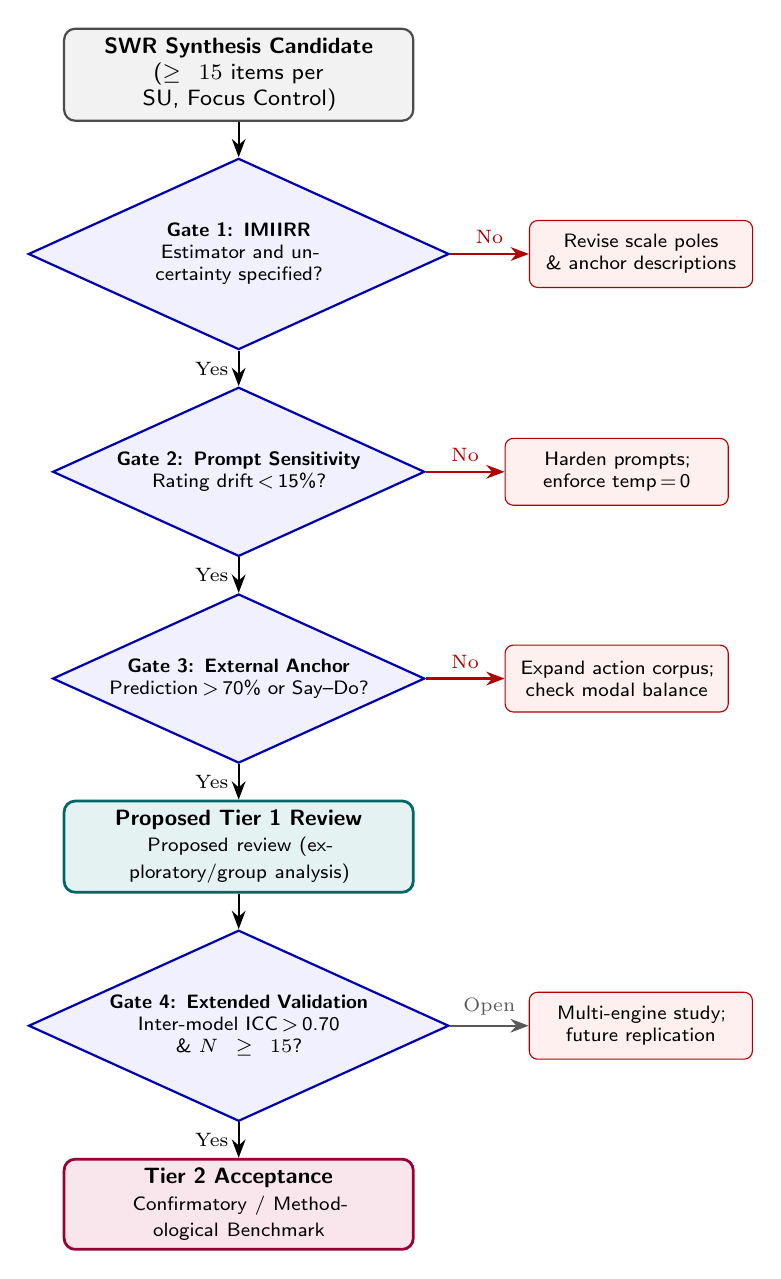
\begin{tikzpicture}[
    >=Stealth,
    node distance=0.45cm and 0.6cm,
    startbox/.style={
      rectangle, rounded corners=4pt, draw=black!70, fill=gray!10!white,
      text width=4.2cm, minimum height=0.75cm, align=center, font=\footnotesize\sffamily, line width=0.8pt
    },
    decision/.style={
      diamond, aspect=2.2, draw=blue!70!black, fill=blue!6!white,
      text width=3.4cm, align=center, font=\scriptsize\sffamily, line width=0.8pt, inner sep=1pt
    },
    failbox/.style={
      rectangle, rounded corners=3pt, draw=red!70!black, fill=red!6!white,
      text width=2.6cm, minimum height=0.85cm, align=center, font=\scriptsize\sffamily
    },
    tier1box/.style={
      rectangle, rounded corners=4pt, draw=teal!80!black, fill=teal!10!white,
      text width=4.2cm, minimum height=0.85cm, align=center, font=\footnotesize\sffamily, line width=1.0pt
    },
    tier2box/.style={
      rectangle, rounded corners=4pt, draw=purple!80!black, fill=purple!10!white,
      text width=4.2cm, minimum height=0.85cm, align=center, font=\footnotesize\sffamily, line width=1.0pt
    }
  ]

    % Main vertical path
    \node[startbox] (start) {\textbf{SWR Synthesis Candidate}\\($\ge 15$ items per SU, Focus Control)};

    \node[decision, below=0.45cm of start] (gate1) {
      \textbf{Gate 1: IMIIRR}\\Estimator and uncertainty specified?
    };

    \node[decision, below=0.45cm of gate1] (gate2) {
      \textbf{Gate 2: Prompt Sensitivity}\\Rating drift\,$<$\,15\%?
    };

    \node[decision, below=0.45cm of gate2] (gate3) {
      \textbf{Gate 3: External Anchor}\\Prediction\,$>$\,70\% or Say--Do?
    };

    \node[tier1box, below=0.45cm of gate3] (t1) {
      \textbf{Proposed Tier 1 Review}\\
      \scriptsize Proposed review (exploratory/group analysis)
    };

    \node[decision, below=0.45cm of t1] (gate4) {
      \textbf{Gate 4: Extended Validation}\\Inter-model ICC\,$>$\,0.70 \& $N \ge 15$?
    };

    \node[tier2box, below=0.45cm of gate4] (t2) {
      \textbf{Tier~2 Acceptance}\\
      \scriptsize Confirmatory / Methodological Benchmark
    };

    % Lateral failure / remediation nodes
    \node[failbox, right=1.0cm of gate1] (remed1) {Revise scale poles\\\& anchor descriptions};
    \node[failbox, right=1.0cm of gate2] (remed2) {Harden prompts;\\enforce temp\,=\,0};
    \node[failbox, right=1.0cm of gate3] (remed3) {Expand action corpus;\\check modal balance};
    \node[failbox, right=1.0cm of gate4] (remed4) {Multi-engine study;\\future replication};

    % Connections
    \draw[->, thick] (start) -- (gate1);
    \draw[->, thick] (gate1) -- node[left, font=\scriptsize] {Yes} (gate2);
    \draw[->, thick] (gate2) -- node[left, font=\scriptsize] {Yes} (gate3);
    \draw[->, thick] (gate3) -- node[left, font=\scriptsize] {Yes} (t1);
    \draw[->, thick] (t1) -- (gate4);
    \draw[->, thick] (gate4) -- node[left, font=\scriptsize] {Yes} (t2);

    \draw[->, thick, red!70!black] (gate1) -- node[above, font=\scriptsize] {No} (remed1);
    \draw[->, thick, red!70!black] (gate2) -- node[above, font=\scriptsize] {No} (remed2);
    \draw[->, thick, red!70!black] (gate3) -- node[above, font=\scriptsize] {No} (remed3);
    \draw[->, thick, gray!70!black] (gate4) -- node[above, font=\scriptsize] {Open} (remed4);

  \end{tikzpicture}}
  \caption{Proposed decision flowchart for tiered quality-assurance review; no empirical gate is passed by this diagram.}
  \label{fig:qa_funnel}\label{fig:qs_trichter}
\end{figure}





\textbf{Tier~1 (proposed checks, not universally validated acceptance criteria):}
\begin{itemize}[nosep]
  \item Within-model repeat agreement: choose the estimator, target measurement, sample design, and uncertainty model before setting a task-specific threshold; the pilot G1/N15 values do not establish a universal ICC $>0.75$ gate.
  \item Prompt sensitivity: $<$\,15\% variation in ratings across semantically equivalent prompt variants.
  \item At least one external anchor: cross-modal prediction, expert validation, or survey comparison.
  \item Instance separation for all measurements contributing to inferential claims.
\end{itemize}

\textbf{Tier~2 (Desirable for methodological contribution):}
\begin{itemize}[nosep]
  \item Inter-model ICC\,$>$\,0.70 (replication with at least one additional frontier model).
  \item Discriminability test: assess whether the method distinguishes prespecified groups, with uncertainty and external meaning still open.
  \item Expected-discrepancy control: a prespecified comparison with a suitable uncertainty model; one synthetic fixture alone does not separate effects from noise.
  \item Repeat-run count and power/uncertainty analysis: specify the target and error model first; the local $N=15$ protocol sets no universal minimum.
\end{itemize}

The pilot documents several proposed checks, but its G1 measurement contract and empirical acceptance status remain open. Inter-model comparison and external construct validation also remain outstanding.


\begin{table}[htbp]
  \centering
  \caption{Two-Tiered Acceptance Matrix for SWR Applications.}
  \label{tab:tiered-acceptance}\label{tab:abgestufte-akzeptanz}
  \scriptsize
  \begin{tabularx}{\textwidth}{@{} l L{2.8cm} L{2.2cm} Y L{2.0cm} @{}}
    \toprule
    \textbf{Tier} & \textbf{Criterion} & \textbf{Target Metric} & \textbf{Addressed Risk / Failure Mode} & \textbf{Pilot Status} \\
    \midrule
    \multirow{4}{*}{Tier 1 (Required)}
    & Intra-Model Reliability (IMIIRR) & Task-specific estimator/uncertainty & Semantic instability; single-run noise & Recorded profiles; gate open \\[3pt]
    & Prompt Sensitivity & Variation $< 15\%$ & Prompt brittleness; phrasing artifact & Completed ($< 10\%$) \\[3pt]
    & External Anchor & Confirmed $\ge 70\%$ & Hallucinatory drift; ungrounded persona & Completed (72\% prediction) \\[3pt]
    & Instance Separation & Fresh instance per run & Context leakage; inflated reliability & Completed (strict) \\
    \midrule
    \multirow{4}{*}{Tier 2 (Desirable)}
    & Inter-Model Replication & Inter-model $\text{ICC} > 0.70$ & Model-family idiosyncrasy & Open (Desideratum) \\[3pt]
    & Group Discriminability & Distinct group profiles & Homogenization; universal LLM prior & Completed (ANOVA / KW) \\[3pt]
    & Expected-Discrepancy Control & Suitable baseline and uncertainty & Spurious say--do gap; aggregation untested & One fixture; gate open \\[3pt]
    & Statistical Power Reserve & Prespecified repeat design & Underpowered variance estimation & One $N=15$ protocol; gate open \\
    \bottomrule
  \end{tabularx}
\end{table}

%% =============================================================================
%% 4. APPLICATION GUIDE
%% =============================================================================
\section{Application Guide}
\label{sec:application}

This section provides a step-by-step guide for researchers who wish to apply SWR to their own populations. The guide assumes familiarity with qualitative research methodology and basic LLM interaction.

Table~\ref{tab:implementation-ledger} and the tiered acceptance matrix (Table~\ref{tab:tiered-acceptance}) condense the guide into an auditable implementation ledger. Its purpose is not to add a new statistical test, but to make explicit which artifact must exist before a reader can evaluate an SWR application as reproducible, minimally validated, and protected against the most common LLM-specific failure modes.

\begin{table}[htbp]
  \centering
  \caption{Minimum Implementation Ledger for a Reproducible SWR Application.}
  \label{tab:implementation-ledger}\label{tab:implementierungsledger}
  \scriptsize
  \begin{tabularx}{\textwidth}{@{} L{2.6cm} Y Y Y @{}}
    \toprule
    \textbf{Workflow object} & \textbf{Required artifact} & \textbf{Minimum gate} & \textbf{Controlled risk} \\
    \midrule
    Population and corpus & Inclusion/exclusion rules plus source, date, and context metadata for each data point & Intersubjectively verifiable group criteria; $\geq$\,15 data points per SU & Ad hoc sampling; unverifiable provenance \\[3pt]
    Synthesis-unit map & Group $\times$ modality $\times$ period matrix with reduction rationale & Each retained SU is linked to a research question; no unmotivated subset duplication & Hidden researcher degrees of freedom \\[3pt]
    Prompt and instance log & Prompt text, model version, temperature, run date, and fresh-instance record & No shared context for reliability, prediction, or say--do measurements & Context leakage; inflated reliability \\[3pt]
    Rating sheet & Dimension definitions, numerical ratings, and data-based justifications & Clearly defined poles; justification for every rating & Opaque scoring; post-hoc interpretation \\[3pt]
    Validation packet & IMIIRR, prompt-sensitivity check, and at least one external anchor & Tier~1 acceptance before inferential claims & Over-reading a single LLM run \\
    \bottomrule
  \end{tabularx}
\end{table}

\subsection{Step~1: Define Population and Collect Data}
\label{sec:app:step1}

\textbf{Define your groups.} SWR operates on sociologically defined groups---not ad hoc clusters. Groups should be defined by observable, intersubjectively verifiable criteria (institutional role, organizational membership, demographic category, ideological stance). Example: ``All CEOs of Fortune~500 tech companies'' is a well-defined group; ``people who secretly believe in transhumanism'' is not.

\textbf{Collect heterogeneous data.} For each group member, collect both statements (interviews, speeches, publications, social media) and actions (decisions, investments, organizational behavior). The duality of statement and action data is methodologically important: it enables say--do comparison (Section~\ref{sec:qa:discrepancy}) and cross-modal prediction (Section~\ref{sec:qa:crossmodal}).

\textbf{Ensure minimum data density.} Aim for $\geq$\,15 data points per synthesis unit. In the pilot study, 20--72 data points per actor (mean: 31.3) supplied the documented group-level syntheses; sufficiency and stability require separate evaluation.

\textbf{Document provenance.} Each data point should carry metadata: source, date, context. A relational database is recommended for managing large corpora. The pilot study used a SQLite database with 9~tables and 5~views.

\subsection{Step~2: Form Synthesis Units}
\label{sec:app:step2}

\textbf{Map the combination space.} List all meaningful group $\times$ modality $\times$ time period combinations. Apply the nine reduction criteria (Section~\ref{sec:method:su}) to reduce this space to a manageable set of core SUs.

\textbf{Prioritize.} Start with the most inclusive SU (all members, all data, entire period) to establish a baseline profile. Then add group-specific SUs for comparison.

\textbf{Pool data directly.} For each SU, concatenate the raw data of all group members into a single chronological dossier. Do not aggregate individual profiles first---the group synthesis should emerge from the pooled evidence.

\subsection{Step~3: Execute the Prompt Protocol}
\label{sec:app:step3}

\textbf{Apply focus control.} Before feeding data to the LLM, replace all identifying information with neutral placeholders. Prepare a blinding script that operates on your specific data format.

\textbf{Maintain instance separation.} Each step that contributes to a distinct measurement must use a fresh LLM instance with no shared context. This is especially critical for:
\begin{itemize}[nosep]
  \item Reliability runs: each replicate is a separate instance.
  \item Cross-modal prediction: predictor and evaluator share no context.
  \item Say--do comparison: statement-based and action-based syntheses are generated independently.
\end{itemize}

\textbf{Set temperature to 0.} This maximizes reproducibility. Even at temperature~0, LLM outputs are not fully deterministic; multi-run reliability testing quantifies the residual variation.

\textbf{Execute the five steps.} For each SU, run the protocol in sequence: data compilation $\to$ synthesis $\to$ structured interview $\to$ meta-reflection $\to$ dimensional rating. Document all prompts and model parameters.

\subsection{Step~4: Define Dimensions and Rate}
\label{sec:app:step4}

\textbf{Design your dimensional system.} The 12~dimensions from the pilot study (Table~\ref{tab:dimensions}) are specific to the AI elite application. For your population, define dimensions that capture the worldview constructs relevant to your research questions. Each dimension should have clearly labeled poles (what does 1~mean? what does 10~mean?) and should be independent of other dimensions to the extent possible.

\textbf{Rate each SU.} Present the synthesized worldview (from Steps~2--4) to a fresh LLM instance along with the dimension definitions. Request a numerical rating for each dimension with justification. The justification serves two purposes: it enables the researcher to verify that the rating reflects the data, and it documents the reasoning for replication.

\textbf{Conduct reliability runs.} For at least one SU, repeat the entire pipeline (Steps~1--5) with $\geq$\,5 independent instances. Compute ICC as the IMIIRR metric. Choose the estimator, target, uncertainty model, and a task-specific threshold before interpreting repeat agreement; a low value may motivate examining dimensional definitions.

\subsection{Step~5: Validate}
\label{sec:app:step5}

\textbf{Minimum validation (Tier~1):} Conduct IMIIRR testing, sensitivity analysis (vary prompt wording), and at least one external anchor. The cross-modal prediction protocol is recommended as the strongest available anchor: derive behavioral predictions from statement data, then evaluate against actual documented actions.

\textbf{Extended validation (Tier~2):} If resources permit, conduct expected-discrepancy control (synthetic control corpus), inter-model replication, and formal power analysis ($N \geq 15$ independent runs).


\subsection{Practical Considerations}
\label{sec:app:practical}

\textbf{Cost and time.} In the pilot study (100~actors, 3,132~data points, 51--56~core SUs, 11~completed validation experiments plus one identified desideratum), the total LLM cost (Claude Opus~4.6 and Claude Sonnet~4.5 via API) was approximately \$200--300 USD. A smaller study (2--5~groups, 200--500~data points) would cost \$20--50 USD. Data collection is the primary time investment; the SWR pipeline itself runs in hours.

\textbf{Common pitfalls.}
\begin{itemize}[nosep]
  \item \emph{Shared context:} Shared context can change repeat comparisons and create spurious effects; the recorded say--do gap differed by 47\% between two protocols, without isolating a causal context effect.
  \item \emph{Leading prompts:} Including group labels (``progressive activists,'' ``conservative voters'') in synthesis prompts invites stereotype reproduction. Use neutral descriptions.
  \item \emph{Dimensional ambiguity:} Poorly defined scale poles are the primary cause of low IMIIRR. Pilot-test your dimensions with 3--5 runs before committing to the full protocol.
  \item \emph{Individual-level temptation:} SWR is designed for group-level analysis. Applying it to individuals reintroduces the contamination risk that the group-level approach structurally avoids.
  \item \emph{Over-interpretation of single runs:} The pilot study showed that single-run estimates deviate from the $N$\,=\,15 mean by MAE\,=\,0.73. Report multi-run averages, not single-run results, for any claim that depends on precise numerical values.
\end{itemize}

\textbf{Transfer sketch: SWR applied to climate scientists.} A researcher studying the collective worldviews of climate scientists (e.g., IPCC authors vs.\ industry-funded researchers) would proceed as follows: (1)~collect public statements (congressional testimonies, op-eds, interviews) and actions (policy recommendations, funding decisions, institutional affiliations) for both groups; (2)~define synthesis units (``IPCC authors, all data'' vs.\ ``industry-funded, all data''); (3)~develop domain-specific dimensions---e.g., \emph{urgency of action} (1\,=\,no rush to 10\,=\,existential emergency), \emph{trust in models} (1\,=\,skeptical to 10\,=\,full confidence), \emph{role of technology} (1\,=\,behavior change to 10\,=\,geoengineering); (4)~run the five-step protocol with instance separation; (5)~compare the two group profiles on the dimensional system. The expected output: two contrasting worldview portraits whose dimensional differences reveal where the groups genuinely disagree vs.\ where they share common ground.


%% =============================================================================
%% 5. COMPARISON WITH RELATED APPROACHES
%% =============================================================================
\section{Positioning: SWR in the Methodological Landscape}
\label{sec:positioning}

SWR occupies a distinct position at the intersection of qualitative and quantitative traditions (Table~\ref{tab:comparison}).

\begin{table}[htbp]
  \centering
  \caption{SWR Compared with Related Methodological Approaches.}
  \label{tab:comparison}
  \footnotesize
  \setlength{\tabcolsep}{5pt}
  \renewcommand{\arraystretch}{1.05}
  \resizebox{\textwidth}{!}{%
  \begin{tabular}{@{} l l l l l l l @{}}
    \toprule
    \textbf{Feature} & \textbf{SWR} & \shortstack[l]{\textbf{Thematic}\\\textbf{Analysis}} & \textbf{Survey} & \shortstack[l]{\textbf{LLM-as-}\\\textbf{Participant}} & \shortstack[l]{\textbf{Automated}\\\textbf{Coding}} & \textbf{CDA} \\
    \midrule
    Data source & \shortstack[l]{Public statements\\+ actions} & \shortstack[l]{Interviews,\\texts} & \shortstack[l]{Direct\\responses} & LLM-generated & \shortstack[l]{Existing\\texts} & \shortstack[l]{Existing\\texts} \\[3pt]
    Unit of analysis & Group & Variable & Individual & \shortstack[l]{Simulated\\individual} & Document & Variable \\[3pt]
    \shortstack[l]{Requires respondent\\access} & No & Yes & Yes & No & No & No \\[3pt]
    Captures coherence & Yes & Partially & No & Limited & No & Partially \\[3pt]
    Scalable & Yes & Limited & Yes & Yes & Yes & Limited \\[3pt]
    External validation & Cross-modal & \shortstack[l]{Member\\checking} & Test--retest & \shortstack[l]{Demographic\\fit} & \shortstack[l]{Expert\\coding} & \shortstack[l]{Analyst\\triangulation} \\[3pt]
    Primary risk & \shortstack[l]{Coherence\\bias} & \shortstack[l]{Researcher\\bias} & \shortstack[l]{Response\\bias} & \shortstack[l]{Stereotype\\reproduction} & \shortstack[l]{Context\\loss} & \shortstack[l]{Small N,\\subjectivity} \\
    \bottomrule
  \end{tabular}}
\end{table}

\textbf{SWR vs.\ Thematic Analysis}~\citep{Braun2006}. Both extract patterns from qualitative data, but thematic analysis identifies themes across a corpus while SWR reconstructs a coherent belief system. The key difference is the coherence constraint: thematic analysis can report contradictory themes side by side; SWR forces them into a single worldview portrait, making tensions visible as internal contradictions rather than separate categories.

\textbf{SWR vs.\ LLM-as-Participant}~\citep{Argyle2023}. LLM-as-Participant generates synthetic data by conditioning the LLM on demographic backstories. SWR compresses real data through LLM-assisted synthesis. The inputs and outputs are fundamentally different: LLM-as-Participant produces survey responses; SWR produces worldview profiles. The contamination structure also differs: LLM-as-Participant draws on training data about demographic groups (by design); SWR structurally avoids this at the group level.

\textbf{SWR vs.\ Automated Coding}~\citep{Tai2024}. Automated coding classifies text segments into predefined categories. SWR goes further by integrating these segments into a coherent whole. Automated coding answers ``what topics are present?''; SWR answers ``what does this group believe?''

\textbf{SWR vs.\ Critical Discourse Analysis}~\citep[CDA;][]{Fairclough1992, Wodak2001}. CDA applies qualitative analytical grids to texts to uncover power structures, ideological formations, and hegemonic discourse patterns. Both CDA and SWR aim to reveal latent belief structures; their relationship is complementary rather than competitive. CDA analyzes individual texts or small corpora on power and ideology; SWR first synthesizes a group-aggregated representation, enabling CDA-style analysis to be applied at the group level rather than the text level. The synthesis pipeline (Steps~1--4) can thus function as a preprocessing stage that makes group-level discourse analysis tractable.

\textbf{Theoretical roots.} SWR draws on~\citet{Weber1904} (ideal type as analytical construct),~\citet{Mannheim1929} (situational determination of thought),~\citet{Gadamer1960} (the hermeneutic circle of understanding), and the sociology-of-knowledge tradition that treats worldviews as social phenomena amenable to empirical investigation~\citep{BergerLuckmann1966}. The emerging field of computational hermeneutics~\citep{Kommers2026} provides a conceptual bridge between these interpretive traditions and LLM-assisted analysis, while~\citet{Hornby2024} examines how Gadamerian hermeneutics can inform the epistemology of LLM-mediated understanding. The inverse-problem formalization connects to~\citet{Tarantola2005} and~\citet{Hadamard1923}. The use of LLMs as analytical instruments aligns with the emerging ``LLMs for social science'' paradigm~\citep{Ziems2024, Bail2024}, while the epistemological caution draws on~\citet{Messeri2024}, who warn of ``illusions of understanding'' when AI tools are deployed without sufficient methodological reflection.


%% =============================================================================
%% 6. LIMITATIONS
%% =============================================================================
\section{Limitations}
\label{sec:limitations}

\subsection{Coherence Bias as Instrument Property}
\label{sec:limitations:coherence}

LLMs are optimized for logical coherence; humans are inherently inconsistent. For worldview reconstruction, this property is both an operational asset and a source of systematic distortion~\citep{Geiger2026PaperA}. The asset: coherence enables SWR to extract a stable, interpretable group-level profile from heterogeneous data---the method \emph{exploits} coherence as a compression mechanism, analogous to how factor analysis exploits covariance structure. The distortion: the resulting worldview types may appear more sharply contoured than they are in reality. Internal tensions that real persons experience---e.g., between power striving and sense of responsibility---risk being resolved by the LLM in favor of a consistent profile.

The genuine limitation is therefore \emph{over-coherence}: clusters sharper than empirical reality. The underlying mechanism is twofold: first, RLHF-driven alignment incentivizes conversational fluency and narrative smoothness, which may lead LLMs to eliminate cognitive dissonances present in the source data; second, the autoregressive generation process builds each token on preceding context, creating a structural tendency toward coherent continuation rather than the representation of genuine ambivalence. These tendencies can produce what might be termed \emph{premature closure}---convergence on a coherent interpretation before the full complexity of the data has been explored.

Four control mechanisms partially address this risk:
\begin{enumerate}[nosep]
  \item The meta-reflection step (Step~4) explicitly instructs the LLM to identify tensions. However, there is no guarantee that this meta-reflection constitutes genuine metacognition rather than an algorithmic simulation thereof---the meta-reflection may reproduce the same coherence biases it is designed to detect.
  \item Outlier detection in the pilot study showed 80--88\% group-level fit, not 100\%, indicating that the model registers and preserves within-group heterogeneity.
  \item The inversion control (constructing anti-persons whose worldview maximally contradicts the data) confirmed that 58\% of dimension-group combinations showed $|\Delta| \geq 5$, demonstrating that the coherent interpretation is a specific, data-supported choice---not the only possible reading.
  \item In the recorded aggregation comparison, 71.7\% of dimension--group combinations in group syntheses lay farther from the midpoint than averaged individual profiles; this local contrast does not establish a general amplification effect.
\end{enumerate}

Despite these measures, coherence bias remains an inherent property of the method. Results should be interpreted as \emph{idealized models} of worldviews---comparable, scalable approximations---not as faithful representations of actual cognitive states. Comparative analyses (between-group differences) are generally more robust than absolute claims about any single group's internal coherence.


\subsection{Contamination and Focus Control Limits}
\label{sec:limitations:contamination}

Even with consistent focus control, it cannot be excluded that the LLM draws on training knowledge---particularly for well-known public figures. Two empirical results constrain this concern: (1)~one placeholder-versus-fictional-name profile comparison yielded $r$\,=\,0.9585 and MAE\,=\,0.33, without an equivalence test; (2)~full identity disclosure (real names) produced only a moderate shift ($r$\,=\,0.850, MAE\,=\,0.67, with the same group average). The group-level design remains an important safeguard (cf.\ Abstract).


\subsection{Circularity Risk}
\label{sec:limitations:circularity}

The SWR pipeline uses the same model family (Claude Opus~4.6) for both synthesis and validation. This raises the question whether validation confirms empirical accuracy or merely the model's internal consistency. However, the concern must be scoped precisely: the recorded Op4b evaluator used a separate instance without shared context, while earlier say--do runs did not always do so. This separation reduces one route for context leakage but does not make the same-model evaluator an independent external validator.

Three recorded design checks inform, but do not resolve, circularity: (1)~G1 and N15 report repeat consistency for fixed profiles, not general instrument stability; (2)~the fictional-control and separately synthesized profiles show descriptive gaps without an estimated noise distribution or proof that fabricated gaps are absent; (3)~cross-modal prediction (Op4) compares LLM-generated predictions with \emph{documented actions} evaluated in the pilot, a limited external modality rather than a full independent validity test. A residual concern applies specifically to the rating step (Op2): the dimensional correlations reported in the pilot study could partly reflect the LLM's internal coherence patterns rather than empirical relationships. This concern is shared by any rating procedure including human raters---a human coder who rates posthumanism high will, by cognitive coherence, also tend to rate locus of control high. External replication by other research groups using different models would strengthen the validity claim but constitutes independent replication, not a prerequisite for any single study's internal coherence.


\subsection{Black-Box Character}
\label{sec:limitations:blackbox}

The LLM's synthesis process is not interpretable at the mechanistic level. The researcher receives an output but cannot trace which specific data points drove which aspects of the synthesis. The dimensional justifications requested in Step~5 provide partial transparency, but the integration logic remains opaque. This is a genuine limitation shared with any LLM-based analysis and mitigated (not eliminated) by multi-run reliability testing: if the instrument produces consistent outputs across independent instances, the black-box process is at least \emph{stable}, even if not fully transparent.


\subsection{Epistemic Risks of LLM Delegation}
\label{sec:limitations:epistemic}

A broader epistemological concern applies to SWR as an instance of LLM-assisted research: the risk of \emph{epistemic freeloading}---outsourcing cognitive labor to AI systems at the expense of the researcher's own epistemic agency. When a researcher delegates the interpretive synthesis of a group's worldview to an LLM, there is a danger that functional output is produced without corresponding understanding. SWR mitigates this risk through its multi-layered design: the researcher must curate the data corpus, define synthesis units, evaluate dimensional scores, and interpret cross-modal discrepancies---activities that require substantive engagement with the material. Nevertheless, researchers should treat LLM-generated reconstructions as hypotheses requiring critical scrutiny rather than as finished analytical products.


\subsection{Temporal and Cultural Boundaries}
\label{sec:limitations:temporal}

SWR reconstructs worldviews from a specific data window. The pilot study covered 2010--2026; the reconstructed worldviews are valid for this period, not beyond. Furthermore, LLMs carry cultural biases from their training data (predominantly English-language, Western, educated sources; cf.~\citealp{Santurkar2023}). For non-Western populations, this bias may distort the synthesis. Researchers working with non-Western groups should consider this limitation and explore model-specific calibration.


\subsection{Open Desiderata}
\label{sec:limitations:desiderata}

Three empirical extensions remain outstanding: (1)~\textbf{Inter-model replication:} demonstrating that the SWR pipeline produces convergent results across different frontier models (e.g., Claude, GPT, Gemini) with strict instance separation. This is analogous to replicating a survey with different interviewer teams and constitutes external replication, not a prerequisite for any single study's validity. (2)~\textbf{Expert validation:} independent domain experts rating the same groups on the same dimensions, providing a human baseline for comparison with LLM-generated profiles. (3)~\textbf{Extended power analysis:} the $N$\,=\,15 validation was conducted on a single synthesis unit; generalization across all SUs requires additional data.


%% =============================================================================
%% 7. ETHICAL CONSIDERATIONS
%% =============================================================================
\section{Ethical Considerations}
\label{sec:ethics}

\subsection{Epistemic Privacy}

SWR raises a novel ethical concern: \emph{epistemic privacy}---the right of individuals and groups to not have their implicit beliefs inferred from public data. Traditional research ethics focus on data collection (informed consent, privacy protection); SWR operates on publicly available data but generates inferences that go beyond what participants explicitly communicated. The worldview profile of a group may reveal collective beliefs that group members would not individually endorse or even recognize.

The group-level design provides a structural safeguard: SWR reports collective patterns, not individual beliefs. No named individual is attributed a specific worldview position. However, for small groups ($n < 10$), the aggregation provides weaker anonymization, and a quasi-individual profile may emerge. Researchers should report group-level findings only for groups large enough to prevent individual identification.

\subsection{Dual-Use Character}

SWR can be used for legitimate purposes (understanding elite belief systems, informing democratic deliberation, analyzing institutional cultures) and for illegitimate ones (profiling political opponents, constructing targeted manipulation campaigns, weaponizing belief-system analysis). This dual-use character is inherent to any method that makes implicit beliefs explicit. The research community should develop norms for responsible SWR use, analogous to the norms governing survey-based opinion research.

\subsection{Recommendations}

\begin{enumerate}[nosep]
  \item Report only group-level findings; do not attribute beliefs to named individuals.
  \item For groups with $n < 10$, explicitly discuss re-identification risk.
  \item Document and publish all prompts and model parameters for full transparency.
  \item Frame results as ``reconstructed belief patterns,'' not as ``what group $X$ really thinks.''
  \item Consider member checking~\citep{SoysalTurkmen2024} as a desideratum when access to group representatives is available.
\end{enumerate}


%% =============================================================================
%% 8. CONCLUSION
%% =============================================================================
\section{Conclusion}
\label{sec:conclusion}

Synthetic Worldview Reconstruction offers a new method for reconstructing the collective belief systems of sociologically defined groups. By formulating worldview analysis as an inverse problem and using LLMs as analytical compression instruments, SWR bridges the gap between qualitative depth and quantitative rigor. The method's distinctive features are:

\begin{enumerate}[nosep]
  \item \textbf{Group-level analysis as default:} SWR is designed for collective belief systems, not individual portraits, and therefore offers a structural contamination advantage (cf.\ Abstract).
  \item \textbf{Dual data modality:} By operating on both statements and actions, SWR enables say--do comparison and cross-modal prediction---validation mechanisms unavailable to methods that rely on a single data type.
  \item \textbf{Consistent instrumentation:} The separate G1 and N15 repeat protocols show local descriptive consistency (rounded G1 group mean 0.902; N15 single-measure coefficient 0.847). Transfer across inputs, matched human comparison, and external validity remain open; prompt documentation supports inspection and repetition.
  \item \textbf{Transferability:} The five-step protocol, the dimensional rating framework, and the tiered acceptance criteria are designed for application to any sociologically defined population---political elites, corporate cultures, religious communities, scientific disciplines. More broadly, the synthesis pipeline (Steps~1--4) is not bound to persons or worldviews: it can serve as an input stage wherever heterogeneous textual evidence needs to be synthesized into a coherent collective representation---including organizational cultures, policy discourses, and historical periods.
\end{enumerate}

The method has been developed and locally explored through a pilot study of 100~influential AI actors~\citep{Geiger2026PaperA}, which generated descriptive group-profile differences and tensions; the claimed aggregation mechanism and external validity remain untested. The present paper abstracts these capabilities into a transferable methodological framework.

SWR does not replace existing methods; it adds a new instrument to the social scientist's toolkit---one that is especially useful when direct access to respondents is unavailable, when public data are abundant, and when the research question targets collective belief systems rather than individual opinions. Its limitations---coherence bias, contamination risk, black-box character, cultural boundaries---are documented and partially controlled; its open desiderata---inter-model replication, expert validation, extended power analysis---define a clear research agenda. The question is not whether LLMs should be used as instruments for social science research, but how they can be used \emph{rigorously}. SWR offers one possible answer.


%% =============================================================================
%% AI DISCLOSURE
%% =============================================================================
\begingroup
\footnotesize
\setstretch{1.0}
\setlength{\parskip}{0pt}
\backmatterlabel{Disclosure Statement: Use of Artificial Intelligence}

\noindent\textbf{AI Disclosure Statement (Extensive).}
This manuscript was prepared with AI-assisted editorial and drafting support from Claude Opus~4.6 (Anthropic; model ID: \texttt{claude-opus-4-6}; accessed via Claude Code CLI, March 2026; temperature~$= 0$; 1M context window). Subsequent verification passes included style and claim calibration via OpenAI Codex/GPT (June~2026) and automated LaTeX, PDF design, and typography verification via Google Antigravity (September~2026); no new data, sources, analyses, or substantive claims were added in these passes. The author designed the method, determined the paper structure, defined all quality criteria, interpreted the results, and retains sole responsibility for all substantive claims, errors, and omissions. The models are not authors or co-authors, are not acknowledged as contributors, and do not function as validation or ground-truth authorities. All validation results reported in this paper originate from the pilot study~\citep{Geiger2026PaperA}, where the methodology for data collection, LLM-assisted synthesis, and statistical analysis is documented in full.


%% =============================================================================
%% DATA AVAILABILITY
%% =============================================================================
\backmatterlabel{Data Availability Statement}

\noindent The pilot study data, analysis scripts, prompt templates, and dimensional definitions are publicly available in the \href{https://github.com/research-line/ai-elite-swr}{project repository}. The repository contains the complete prompt library, the $100 \times 12$ rating matrix, and all validation analysis scripts.


%% =============================================================================
%% LICENSE
%% =============================================================================
\backmatterlabel{License}

\noindent This work is licensed under the Creative Commons Attribution 4.0 International License (CC-BY-4.0). The full license text is available on the \href{https://creativecommons.org/licenses/by/4.0/}{CC-BY-4.0 license page}.
\endgroup


%% =============================================================================
%% BIBLIOGRAPHY
%% =============================================================================
\newpage

\bibliographystyle{plainnat}
\begin{thebibliography}{99}

\bibitem[Argyle et~al.(2023)]{Argyle2023}
  Argyle, L.~P., Busby, E.~C., Fulda, N., Gubler, J.~R., Rytting, C.~\& Wingate, D. (2023).
  Out of One, Many: Using Language Models to Simulate Human Samples.
  \textit{Political Analysis}, \textit{31}(3), 337--351. \url{https://doi.org/10.1017/pan.2023.2}.

\bibitem[Bail(2024)]{Bail2024}
  Bail, C.~A. (2024).
  Can Generative AI improve social science?
  \textit{Proceedings of the National Academy of Sciences}, \textit{121}(21), Article~e2314021121. \url{https://doi.org/10.1073/pnas.2314021121}.

\bibitem[Barros et~al.(2024)]{Barros2024}
  Barros, C.\,F., Azevedo, B.\,B., Graciano Neto, V.\,V., Kassab, M., Kalinowski, M., do Nascimento, H.\,A.\,D.~\& Bandeira, M.\,C.\,G.\,S.\,P. (2024).
  Large Language Model for Qualitative Research---A Systematic Mapping Study.
  \textit{arXiv:2411.14473}. \url{https://arxiv.org/abs/2411.14473}.

\bibitem[Berger \& Luckmann(1966)]{BergerLuckmann1966}
  Berger, P.~L.~\& Luckmann, T. (1966).
  \textit{The Social Construction of Reality}.
  New York: Doubleday.

\bibitem[Bourdieu(1977)]{Bourdieu1977}
  Bourdieu, P. (1977).
  \textit{Outline of a Theory of Practice}.
  Cambridge University Press.

\bibitem[Braun \& Clarke(2006)]{Braun2006}
  Braun, V.~\& Clarke, V. (2006).
  Using thematic analysis in psychology.
  \textit{Qualitative Research in Psychology}, \textit{3}(2), 77--101. \url{https://doi.org/10.1191/1478088706qp063oa}.

\bibitem[Fairclough(1992)]{Fairclough1992}
  Fairclough, N. (1992).
  \textit{Discourse and Social Change}.
  Cambridge: Polity Press.

\bibitem[Fugard \& Potts(2015)]{FugardPotts2015}
  Fugard, A.~J.~B.~\& Potts, H.~W.~W. (2015).
  Supporting thinking on sample sizes for thematic analyses: A quantitative tool.
  \textit{International Journal of Social Research Methodology}, \textit{18}(6), 669--684. \url{https://doi.org/10.1080/13645579.2015.1005453}.

\bibitem[Gadamer(1960)]{Gadamer1960}
  Gadamer, H.-G. (1960).
  \textit{Wahrheit und Methode}.
  Tübingen: Mohr.

\bibitem[Ge et~al.(2024)]{Ge2024}
  Ge, T.~et~al. (2024).
  Scaling synthetic data creation with 1{,}000{,}000{,}000 personas.
  \textit{arXiv:2406.20094}. \url{https://arxiv.org/abs/2406.20094}.

\bibitem[Geiger(2026)]{Geiger2026PaperA}
  Geiger, L. (2026).
  What does the AI elite think? A synthetic worldview reconstruction of the 100 most influential AI actors (2010--2026).
  Zenodo. \url{https://doi.org/10.5281/zenodo.18736737}.

\bibitem[Guest et~al.(2006)]{Guest2006}
  Guest, G., Bunce, A.~\& Johnson, L. (2006).
  How many interviews are enough? An experiment with data saturation and variability.
  \textit{Field Methods}, \textit{18}(1), 59--82. \url{https://doi.org/10.1177/1525822X05279903}.

\bibitem[Hadamard(1923)]{Hadamard1923}
  Hadamard, J. (1923).
  \textit{Lectures on Cauchy's Problem in Linear Partial Differential Equations}.
  New Haven: Yale University Press.

\bibitem[Hallgren(2012)]{Hallgren2012}
  Hallgren, K.~A. (2012).
  Computing Inter-Rater Reliability for Observational Data: An Overview and Tutorial.
  \textit{Tutorials in Quantitative Methods for Psychology}, \textit{8}(1), 23--34. \url{https://doi.org/10.20982/tqmp.08.1.p023}.

\bibitem[Hornby(2025)]{Hornby2024}
  Hornby, R. (2025).
  Is Generative AI Ready to Join the Conversation That We Are?
  \textit{Technophany: A Journal for Philosophy and Technology}, \textit{3}(1), 1--31. \url{https://doi.org/10.54195/technophany.18134}.

\bibitem[Kommers et~al.(2026)]{Kommers2026}
  Kommers, C., Ahnert, R., Antoniak, M., Benetos, E., Benford, S., Bunz, M.~et~al. (2026).
  Computational Hermeneutics: Evaluating Generative AI as a Cultural Technology.
  \textit{Frontiers in Artificial Intelligence}, \textit{9}, Article~1753041. \url{https://doi.org/10.3389/frai.2026.1753041}.

\bibitem[Mannheim(1929)]{Mannheim1929}
  Mannheim, K. (1929).
  \textit{Ideologie und Utopie}.
  Bonn: Cohen.

\bibitem[Messeri \& Crockett(2024)]{Messeri2024}
  Messeri, L.~\& Crockett, M.~J. (2024).
  Artificial intelligence and illusions of understanding in scientific research.
  \textit{Nature}, \textit{627}, 49--58. \url{https://doi.org/10.1038/s41586-024-07146-0}.

\bibitem[Norman(2010)]{Norman2010}
  Norman, G. (2010).
  Likert scales, levels of measurement and the ``laws'' of statistics.
  \textit{Advances in Health Sciences Education}, \textit{15}(5), 625--632. \url{https://doi.org/10.1007/s10459-010-9222-y}.

\bibitem[Ornstein et~al.(2025)]{Ornstein2025}
  Ornstein, J.~T., Blasingame, E.~N.~\& Truscott, J.~S. (2025).
  How to Train Your Stochastic Parrot: Large Language Models for Political Texts.
  \textit{Political Science Research and Methods}, \textit{13}(2), 264--281. \url{https://doi.org/10.1017/psrm.2024.64}.

\bibitem[Santurkar et~al.(2023)]{Santurkar2023}
  Santurkar, S., Durmus, E., Ladhak, F., Lee, C., Liang, P.~\& Hashimoto, T. (2023).
  Whose opinions do language models reflect?
  In: \textit{Proceedings of the 40th International Conference on Machine Learning}, PMLR~202, 29971--30004. \url{https://proceedings.mlr.press/v202/santurkar23a.html}.

\bibitem[Soysal \& Türkmen(2024)]{SoysalTurkmen2024}
  Soysal, Y.~\& Türkmen, S. (2024).
  Reinterpreting the Member Checking Validation Strategy in Qualitative Research Through the Hermeneutics Lens.
  \textit{Qualitative Inquiry in Education: Theory \& Practice}, \textit{2}(1), 42--63. \url{https://doi.org/10.59455/qietp.19}.

\bibitem[Tai et~al.(2024)]{Tai2024}
  Tai, R.~H.~et~al. (2024).
  An Examination of the Use of Large Language Models to Aid Analysis of Textual Data.
  \textit{International Journal of Qualitative Methods}, \textit{23}, Article~16094069241231168. \url{https://doi.org/10.1177/16094069241231168}.

\bibitem[Tarantola(2005)]{Tarantola2005}
  Tarantola, A. (2005).
  \textit{Inverse Problem Theory and Methods for Model Parameter Estimation}.
  Philadelphia: SIAM.

\bibitem[Trope \& Liberman(2010)]{TropeLiberman2010}
  Trope, Y.~\& Liberman, N. (2010).
  Construal-Level Theory of Psychological Distance.
  \textit{Psychological Review}, \textit{117}(2), 440--463. \url{https://doi.org/10.1037/a0018963}.

\bibitem[Wang et~al.(2025)]{Wang2025}
  Wang, Q., Erqsous, M., Barner, K.~E.~\& Mauriello, M.~L. (2025).
  LATA: A Pilot Study on LLM-Assisted Thematic Analysis of Online Social Network Data Generation Experiences.
  \textit{Proceedings of the ACM on Human-Computer Interaction}, \textit{9}(2), Article~124, 1--28. \url{https://doi.org/10.1145/3711022}.

\bibitem[Weber(1904)]{Weber1904}
  Weber, M. (1904).
  Die ``Objektivität'' sozialwissenschaftlicher und sozialpolitischer Erkenntnis.
  \textit{Archiv für Sozialwissenschaft und Sozialpolitik}, \textit{19}, 22--87.

\bibitem[Wodak \& Meyer(2001)]{Wodak2001}
  Wodak, R.~\& Meyer, M. (Eds.) (2001).
  \textit{Methods of Critical Discourse Analysis}.
  London: Sage.

\bibitem[Ziems et~al.(2024)]{Ziems2024}
  Ziems, C., Held, W., Shaikh, O., Chen, J., Zhang, Z.~\& Yang, D. (2024).
  Can Large Language Models Transform Computational Social Science?
  \textit{Computational Linguistics}, \textit{50}(1), 237--291. \url{https://doi.org/10.1162/coli_a_00502}.

\end{thebibliography}


%% =============================================================================
%% APPENDIX
%% =============================================================================
\newpage
\appendix

\section{Prompt Templates}
\label{app:prompts}

The following templates illustrate the five-step protocol. All prompts used in the pilot study are archived in the repository (\url{https://github.com/research-line/ai-elite-swr}).

\subsection{Step~2: Synthesis Prompt (Op1)}

\begin{promptquote}
You receive a collection of anonymized statements and actions from a group of persons. Your task is to construct a fictional person whose worldview best explains the totality of the presented data. This person does not exist---they are an analytical construct that distills the group's collective beliefs.

Describe this person's:

1. Self-image: Who are they? What drives them? How do they see their role?

2. Worldview: How does the world work? What forces shape the future? What is the role of technology, power, and institutions?

3. View of humanity: What is the nature of human beings? What are their strengths and limitations? Can they be improved?

Also identify: Internal tensions, blind spots, and beliefs this person holds without being aware of them.

[Data corpus follows]
\end{promptquote}

\subsection{Step~5: Rating Prompt (Op2)}

\begin{promptquote}
You receive a collection of anonymized statements and actions from a group of persons in a professional domain. Based on these data, assess the collective worldview of the group on the following 12 dimensions (scale 1--10). Justify each assessment with concrete references to the data points.

[Followed by: dimension definitions D01--D12 with scale poles, then the anonymized data corpus.]
\end{promptquote}

\subsection{Cross-Modal Prediction Prompts (Op4)}

\textbf{Op4a (Prediction):}
\begin{promptquote}
You receive the public statements of a group of persons. Based ONLY on these statements, predict 10 concrete actions you would expect from this group. Be specific: what investments, decisions, organizational changes, or political activities would follow from these stated beliefs?

[Statement corpus follows]
\end{promptquote}

\textbf{Op4b (Evaluation):}
\begin{promptquote}
You receive two inputs: (1) a list of 10 predicted actions and (2) the documented real actions of a group of persons. For each prediction, assess: Is it CONFIRMED by the real actions, PLAUSIBLE but without direct match, or CONTRADICTED?

[Predictions + action corpus follow]
\end{promptquote}


\section{Glossary}
\label{app:glossary}

\begin{description}[style=nextline, leftmargin=2cm]
  \item[DV] Dependent Variable. SWR defines three: DV1 (self-image), DV2 (worldview), DV3 (view of humanity).
  \item[Focus Control] The ensemble of measures ensuring LLM task compliance: anonymization + task-focused prompting.
  \item[IMIIRR] Intra-Model Inter-Instance Rating Reliability. The consistency of ratings across independent LLM instances processing the same data.
  \item[Instance Separation] The requirement that each measurement contributing to an inferential claim uses a fresh LLM instance with no shared context.
  \item[Op1--Op6] Operationalizations defined in the SWR framework. Op1: core synthesis; Op2: dimensional rating; Op4: cross-modal prediction; Op5: bottom-up clustering; Op6: structured dialogue. Op3 (text analysis) was defined but not implemented in the pilot study. Op5 was implemented as PCA + HDBSCAN on the $100 \times 12$ rating matrix (not as Sentence-BERT clustering as originally conceived).
  \item[SU] Synthesis Unit. The atomic unit of SWR analysis: a specific group $\times$ modality $\times$ time period combination processed through the five-step protocol.
  \item[SWR] Synthetic Worldview Reconstruction. The method described in this paper.
\end{description}


\end{document}
